\section{Penelitian dan Riset Terkait}
\label{sec:penelitian-riset-terkait}

Berikut merupakan riset dan penelitian yang selaras dan juga menjadi komponen pendukung bagi tugas akhir ini.

% ekstraksi data
\subsection{Extraction, indexing, and analysis of Ethereum Smart Contracts data}
\label{subsec:extraction-indexing-analysis-ethereum-sc}

\begin{figure}[ht]
	\centering
	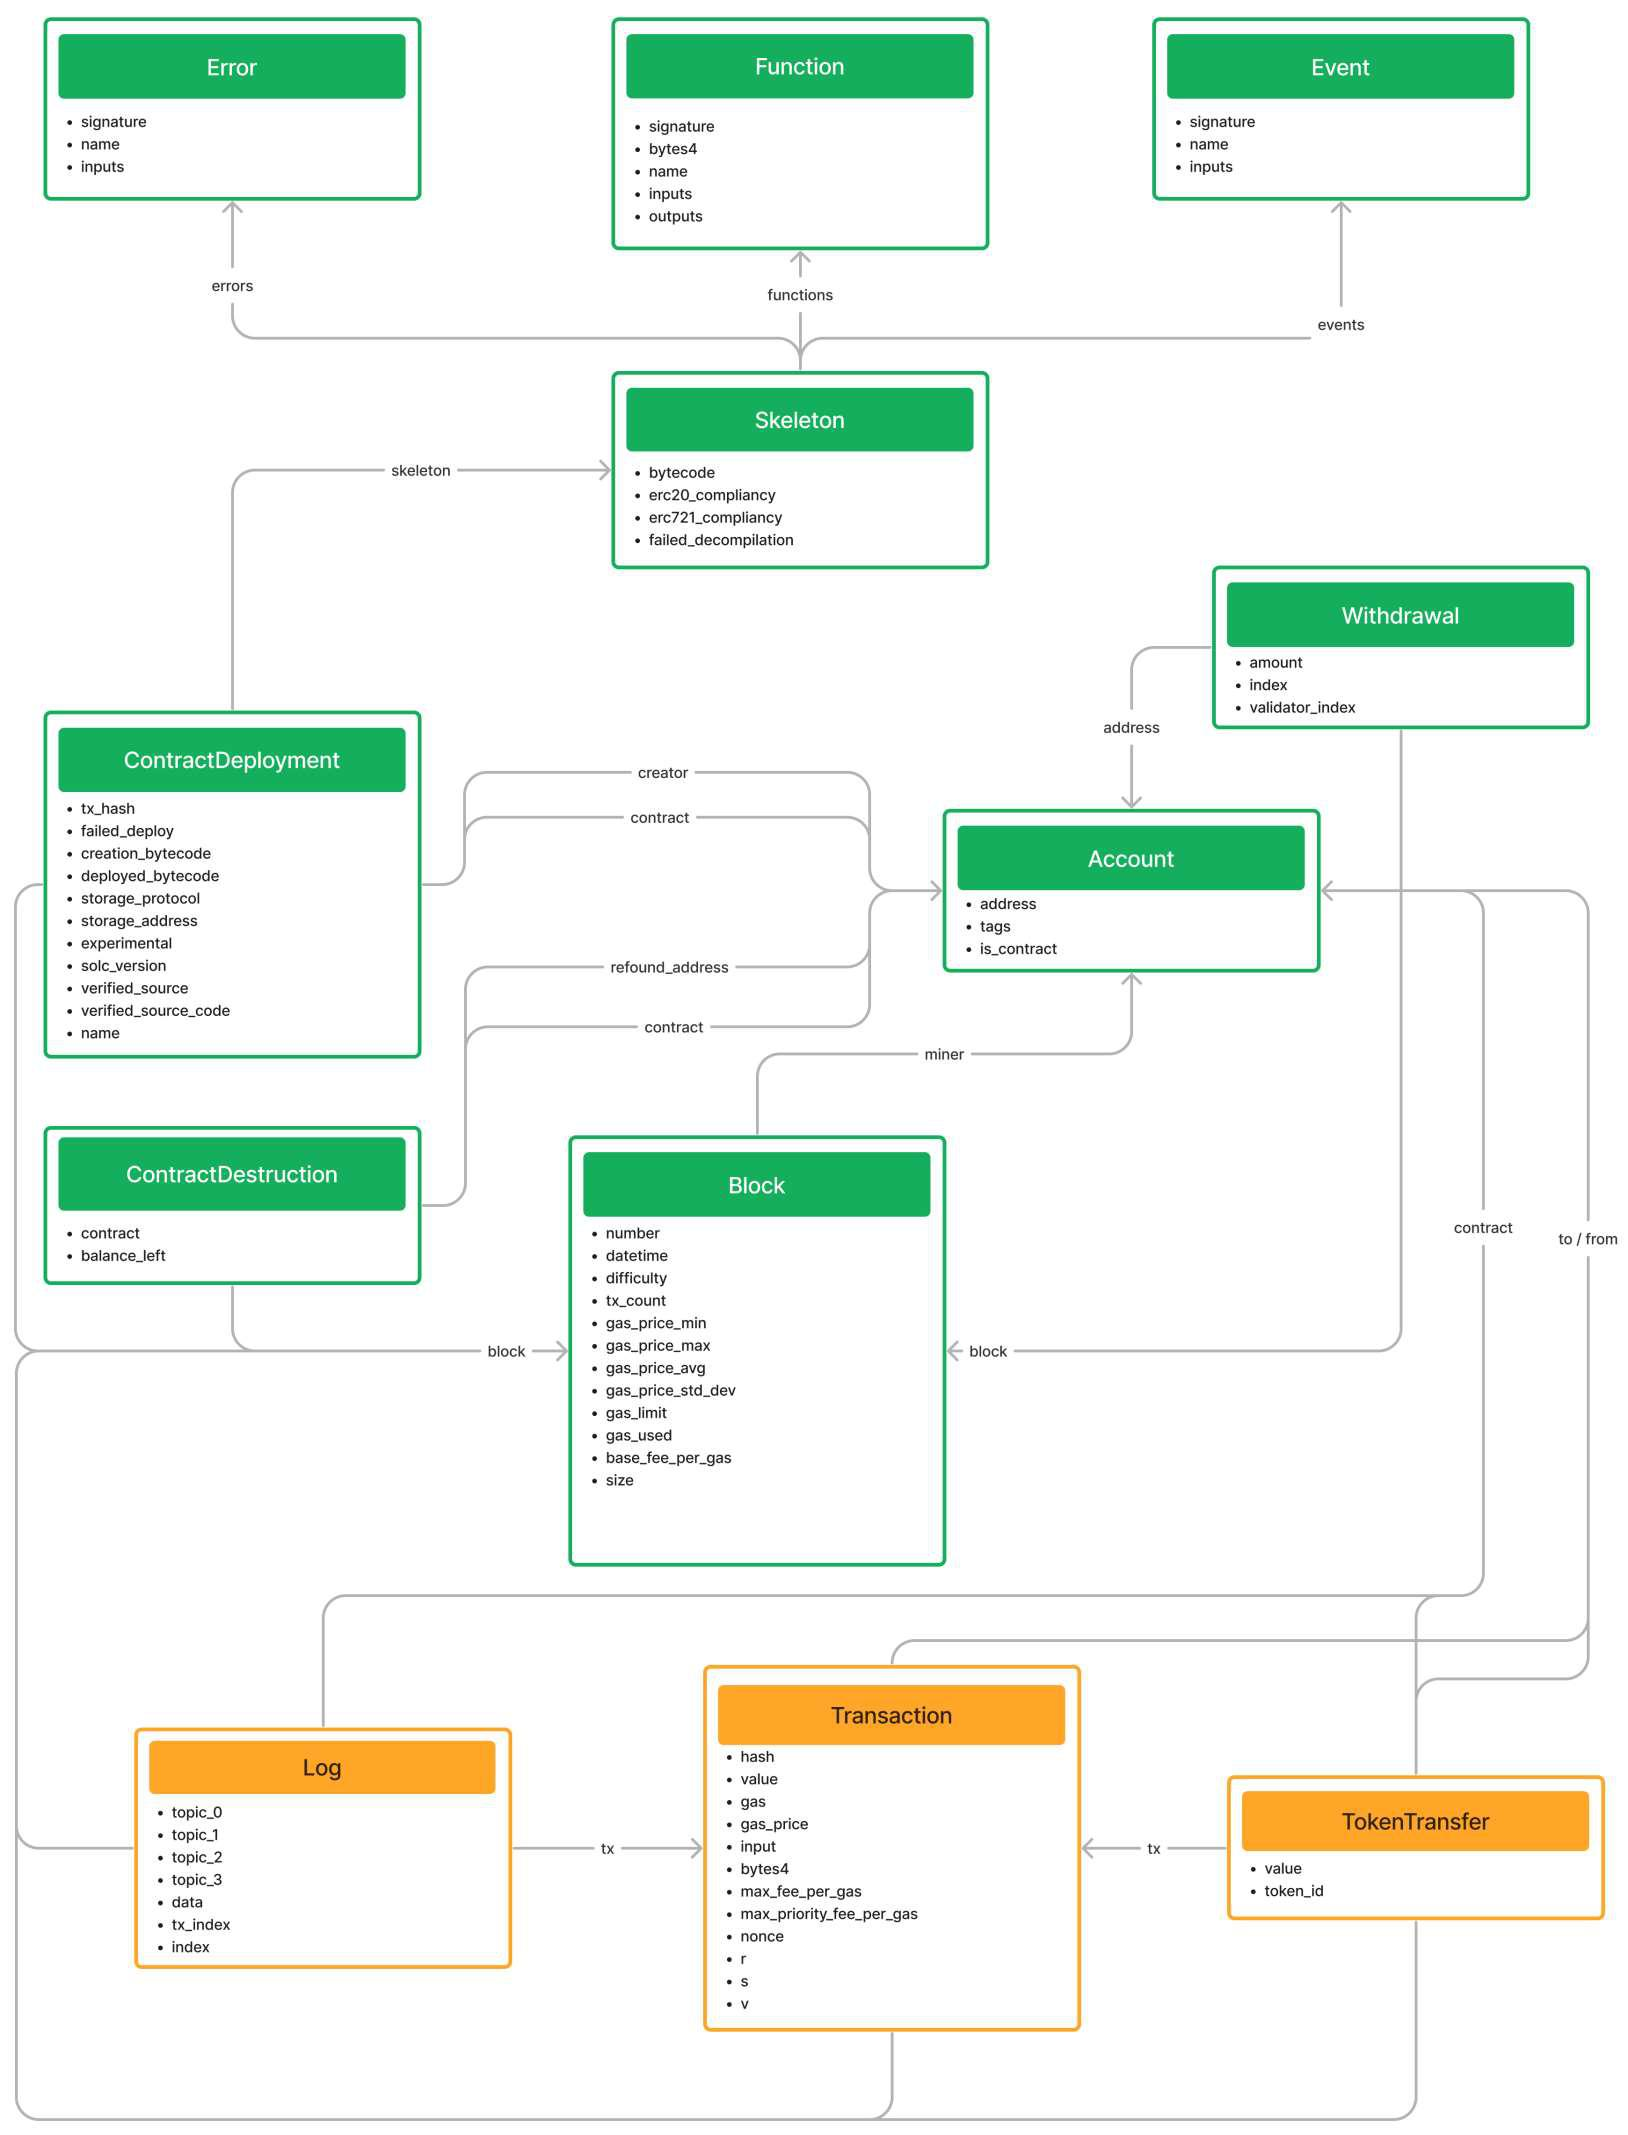
\includegraphics[width=0.7\textwidth]{resources/chapter-2/eth2dgraph-structure.jpg}
	\caption{Data model eth2dgraph \parencite{aimar2023extraction}}
	\label{image:eth2dgraph-structure}
\end{figure}

Penelitian yang dilakukan sebagai \textit{thesis} oleh \cite{aimar2023extraction} berfokus pada bagaimana mengambil data dari Blockchain Ethereum yang bersifat publik, mengekstrasi semantiknya, lalu mentransformasikannya ke sebuah bentuk yang mudah diakses oleh pengguna dengan cara mengindeksnya menggunakan Dgraph, sebuah \textit{open-source distributed graph database}. Hasil dari penelitian ini adalah sebuah perangkat lunak bernama eth2dgraph, yang ditulis dalam bahasa Rust yang melakukan mapping data Ethereum ke format Dgraph, dengan data model yang ditunjukkan pada gambar \ref{image:eth2dgraph-structure}. Perangkat lunak ini mengintegrasikan sebuah \textit{decompiler} untuk mengekstraksi dan mengindeks ABI dari Smart Contracts.

Beberapa hal yang dapat diperhatikan dari perangkat lunak eth2dgraph adalah:

\begin{enumerate}
	\item Ekstraksi ABI \newline Cara eth2dgraph mengekstraksi semantik dari sebuah Smart Contract yang sudah dalam bentuk EVM Bytecode, yaitu dalam ABI (\textit{Application Binary Interface}). Gambar \ref{image:abi-extraction} menggambarkan bagaimana eth2dgraph memanfaatkan heimdall-rs untuk melakukan dekompilasi ABI. Cara ini dapat mengekstraksi lokasi fungsi, informasi terkait tipe \textit{input} dan \textit{output} dan nama fungsi, tetapi tidak memungkinkan untuk mengekstraksi nama parameter karena sudah dihilangkan pada saat kompilasi.
	      \begin{figure}[ht]
		      \centering
		      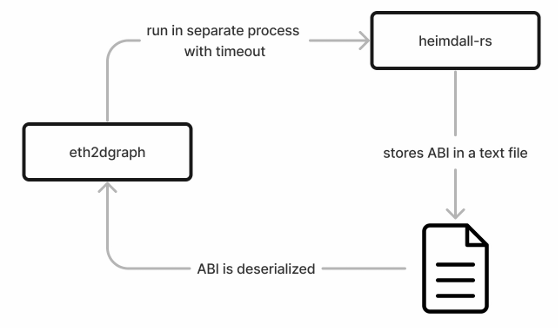
\includegraphics[width=0.7\textwidth]{resources/chapter-2/eth2dgraph-heimdall.png}
		      \caption{Ekstraksi ABI \parencite{aimar2023extraction}}
		      \label{image:abi-extraction}
	      \end{figure}
	\item Ekstraksi struktur dan metadata \newline Cara eth2dgraph mengekstraksi struktur Smart Contract dan metadata adalah menggunakan Regular Expression, dengan bagian \textit{runtime} diproses untuk mengekstraksi struktur, sedangkan bagian metadata dilakukan \textit{decode}.
	\item Ekstraksi menggunakan source code \newline eth2dgraph juga dapat melakukan ekstraksi semantik menggunakan source code yang tersedia dari sebuah Smart Contract, dengan cara melakukan query terhadap teks yang ada di dalam Smart Contract.
\end{enumerate}

\subsection{Ethereum ETL}
\label{subsec:ethereum-etl}

Ethereum ETL (Extract, Transform, Load) adalah sebuah kakas yang dirancang untuk mengekstraksi, mentransformasi, dan memuat data dari blockchain Ethereum. Kakas ini ditujukan bagi pengembang dan analis yang ingin mengakses serta memproses data blockchain, memungkinkan integrasi ke dalam basis data atau alat analisis lainnya. 

Dikembangkan oleh tim Blockchain ETL, sistem ini menyediakan serangkaian alat untuk:

\begin{enumerate}
  \item Ekspor Data Ethereum: Mendukung ekspor blok Ethereum, transaksi, transfer token ERC20/ERC721, transaksi internal, log, dan data kontrak ke dalam format yang mudah diakses seperti file CSV atau basis data relasional.
  \item Streaming Data: Ethereum ETL memungkinkan streaming data blockchain secara \textit{real-time}, memberikan akses langsung ke transaksi, blok, dan transfer token Ethereum.
  \item Integrasi BigQuery: Pustaka ini menyediakan cara mudah untuk mengunggah dan menjalankan kueri terhadap data Blockchain Ethereum melalui Google BigQuery, memfasilitasi analisis data dalam skala besar.
\end{enumerate}

Arsitektur sistem yang dirancang untuk fleksibilitas memungkinkan pengguna untuk mengatur pekerjaan ETL untuk kumpulan data Ethereum, dan menyediakan cara yang efisien untuk menganalisis atau memvisualisasikan data Blockchain. Sebagai \textit{open-source software}, Ethereum ETL membantu pengguna berinteraksi dengan data Ethereum tanpa memerlukan pengaturan infrastruktur Blockchain yang kompleks. \parencite{ethereum_etl}
\subsection{Xblock-ETH}
\label{subsec:xblock-eth}

\cite{zheng2020xblock} mempublikasikan sebuah \textit{dataset} data mentah dari Blockchain Ethereum, dan mengusulkan sebuah \textit{framework} yang digunakan untuk mendapatkan data tersebut, yang disebut Xblock-ETH. Data dilakukan \textit{update} secara periodik dalam \textit{chunk} berjumlah 500,000 blok. \textit{Dataset} ini terbagi menjadi beberapa \textit{dataset} yang lebih kecil yang meliputi: \textit{block}, \textit{block transaction}, \textit{internal transaction}, \textit{contract info}, \textit{ERC20 transaction}, \textit{ERC721 transaction}, dan \textit{token info}.

Xblock-ETH menyediakan alternatif untuk mendapatkan data tanpa menjalankan sebuah \textit{node} Ethereum, yang memerlukan waktu dan sumber daya yang besar. Tetapi kekurangan dari Xblock-ETH adalah terdapat kekurangan informasi yang penting seperti \textit{logs} dan \textit{receipts}. Secara penggunaan, Xblock-ETH dinilai kurang mudah untuk digunakan karena memerlukan \textit{parsing} data CSV yang banyak, yang tidak mudah dilakukan query atau \textit{index}.


\subsection{Sourcify}
\label{subsec:sourcify}

Sourcify adalah sebuah inisiatif dan layanan \textit{open source} yang bertujuan untuk menyediakan repositori publik dan terdesentralisasi untuk \textit{source code} dari Smart Contracts. Layanan ini mendukung berbagai blockchain yang kompatibel dengan Ethereum Virtual Machine (EVM), termasuk Ethereum, Polygon, Binance Smart Chain, dan Avalanche. Tujuan utama Sourcify adalah meningkatkan transparansi dan kepercayaan dalam ekosistem Smart Contract dengan memungkinkan verifikasi \textit{source code} secara independen.

Proses verifikasi di Sourcify sangat bergantung pada \textit{metadata} kontrak, yang biasanya berupa file JSON yang dihasilkan oleh \textit{compiler} (misalnya, Solidity atau Vyper). File metadata ini berisi informasi krusial seperti versi \textit{compiler}, pengaturan optimasi, dan \textit{hash} dari setiap file \textit{source code}. Sourcify menggunakan informasi ini untuk merekompilasi \textit{source code} yang diajukan dan membandingkan \textit{bytecode} yang dihasilkan dengan \textit{bytecode} yang ada di blockchain.

Sourcify membedakan dua tingkat pencocokan utama:
\begin{itemize}
	\item \textbf{Full Match (Pencocokan Penuh):} Dianggap sebagai standar verifikasi tertinggi. Terjadi ketika \textit{bytecode} yang dihasilkan dari rekompilasi identik dengan \textit{bytecode} on-chain, dan \textit{hash} dari file metadata (yang biasanya ditambahkan di akhir \textit{bytecode} oleh \textit{compiler} Solidity) juga cocok. Ini memberikan jaminan kriptografis bahwa \textit{source code} yang diverifikasi, termasuk komentar dan nama variabel, adalah sama persis dengan yang digunakan saat \textit{deployment}.
	\item \textbf{Partial Match (Pencocokan Sebagian):} Terjadi ketika \textit{bytecode} yang direkompilasi cocok dengan \textit{bytecode} on-chain, tetapi \textit{hash} metadatanya mungkin berbeda. Ini menunjukkan bahwa fungsionalitas kontrak kemungkinan besar sama, namun bisa terdapat perbedaan kosmetik pada \textit{source code} (misalnya, komentar atau spasi). Tingkat verifikasi ini serupa dengan yang umum ditemukan pada platform block explorer seperti Etherscan.
\end{itemize}

Untuk mendukung aspek desentralisasinya, Sourcify sering memanfaatkan InterPlanetary File System (IPFS) untuk menyimpan dan menyebarkan \textit{source code} serta metadata yang terverifikasi. Seluruh repositori data Sourcify juga dapat diakses dan diunduh untuk keperluan analisis dan penelitian lebih lanjut, yang terdiri dari basis data berisi \textit{source code}, \textit{bytecode}, metadata, dan detail \textit{deployment} dari kontrak-kontrak yang telah terverifikasi \parencite{sourcify_website}.

% pemodelan, penyimpanan, indexing
\subsection{Linked Data Indexing of Distributed Ledgers}
\label{subsec:linked-data-indexing-distributed-ledgers}

Penelitian yang dilakukan oleh \cite{third2017linked} membahas tantangan dalam pencarian informasi pada \textit{distributed ledger}, yang sulit dilakukan karena informasi mengenai suatu entitas dapat tersebar di seluruh \textit{ledger} tanpa adanya indeks. Penelitian ini mengusulkan penggunaan indeks berbasis semantik untuk Ethereum Blockchain dengan pendekatan \textit{Linked Data}, yang memungkinkan pencarian menggunakan istilah khusus sesuai \textit{domain}. Pendekatan ini diharapkan dapat meningkatkan kekuatan, kegunaan, dan cakupan dari sistem \textit{ledger} tersebut.

Dalam penelitian ini, mereka mengimplementasikan indeks semantik pada Ethereum Blockchain untuk mengekspos data di dalam \textit{distributed ledger} sebagai \textit{Linked Data}. Indeks ini mengindeks data pada level blok dan transaksi menggunakan ontologi BLONDiE, serta memetakan Smart Contract ke dalam ontologi \textit{Minimal Service Model} (MSM) sebagai langkah awal untuk menghubungkan Smart Contract dengan \textit{Semantic Web Services}.

Implementasi indeks semantik ini menggunakan ontologi BLONDiE sebagai kerangka untuk mengelompokkan dan mendeskripsikan elemen-elemen utama dari Blockchain. Ontologi \textit{Minimal Service Model}, yang biasanya digunakan untuk \textit{web services}, diterapkan untuk menggambarkan fungsionalitas dari Smart Contract pada Blockchain, sehingga memungkinkan integrasi yang lebih efisien.

\begin{figure}[ht]
  \centering
  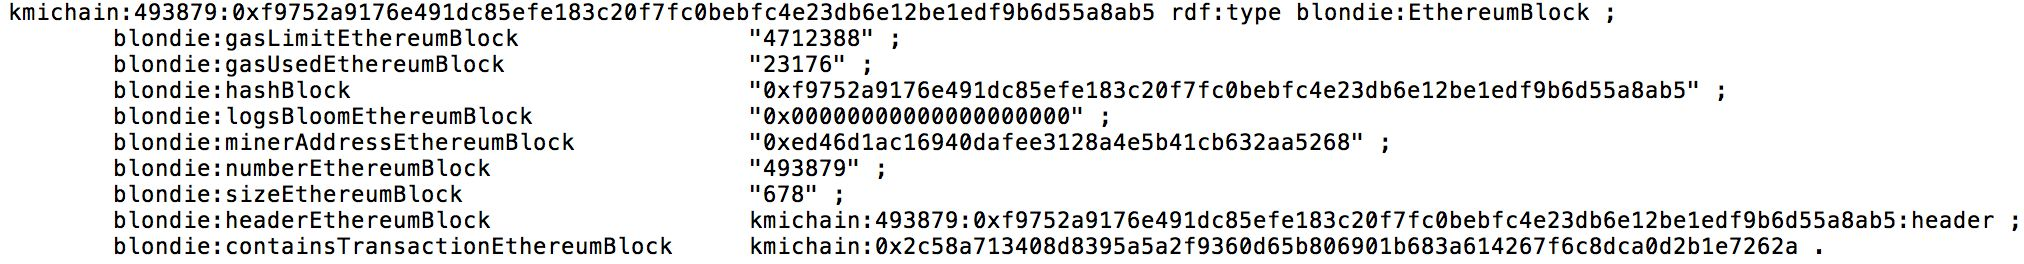
\includegraphics[width=1\textwidth]{resources/chapter-2/rdf-block.jpg}
  \caption{RDF dari deskripsi blok \parencite{third2017linked}}
  \label{image:rdf-block}
\end{figure}

\begin{figure}[ht]
  \centering
  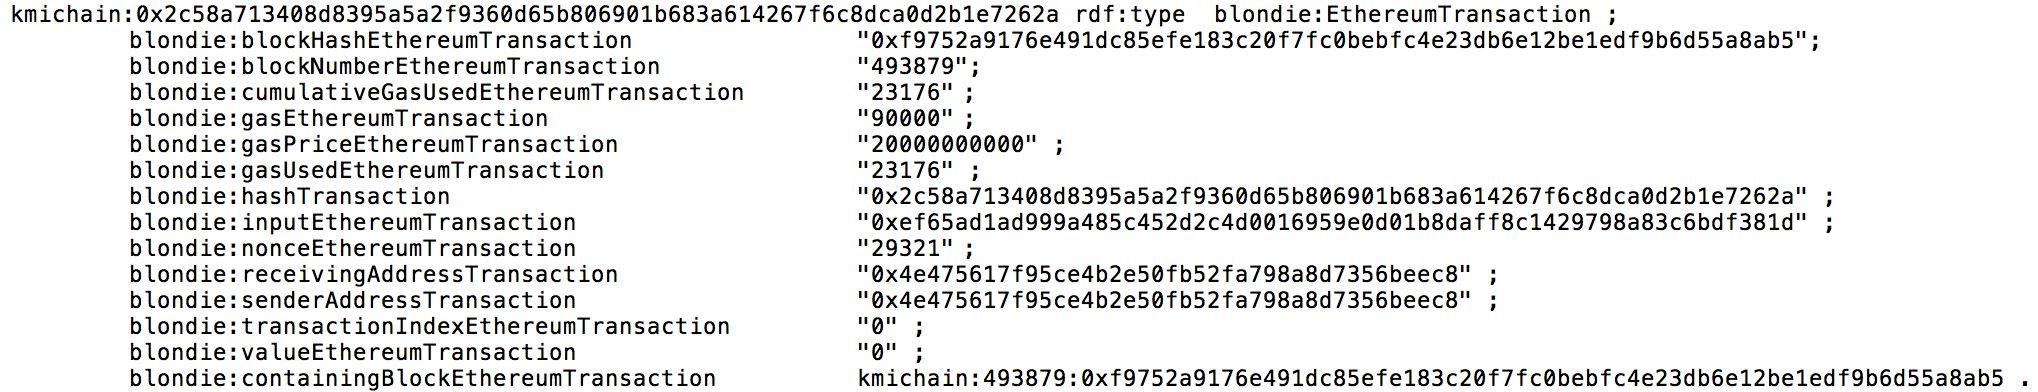
\includegraphics[width=1\textwidth]{resources/chapter-2/rdf-transaction.jpg}
  \caption{RDF dari deskripsi transaksi \parencite{third2017linked}}
  \label{image:rdf-transaction}
\end{figure}

Proyek ini diimplementasikan pada jaringan Ethereum Blockchain privat, di mana komponen \textit{listener} dikembangkan untuk mendeteksi blok baru dan mengindeksnya berdasarkan ontologi BLONDiE. RDF \textit{triples} kemudian dihasilkan dari data ini, yang memungkinkan penguraian data Blockchain secara semantik untuk mendukung pencarian data yang lebih terstruktur. Gambar \ref{image:rdf-block} dan gambar \ref{image:rdf-transaction} adalah contoh dari RDF \textit{triples} yang dihasilkan dari deskripsi blok dan transaksi masing-masing.

Hasil dari penelitian ini menunjukkan bahwa \textit{semantic indexing} memungkinkan data di dalam Blockchain menjadi lebih mudah diakses dan dapat terintegrasi dengan sumber data eksternal. Hal ini membuka peluang untuk mengembangkan \textit{semantic indexing} pada platform Blockchain lainnya serta berpotensi memperluas interoperabilitas data antara Blockchain dan \textit{Semantic Web}.
\subsection{The Graph Protocol}
\label{subsec:the-graph-protocol}

Produk yang dikembangkan oleh \cite{TheGraphDocs}, The Graph, adalah sebuah protokol indeksasi terdesentralisasi untuk data blockchain yang memungkinkan pengguna untuk mendapatkan data terstruktur dari blockchain lainnya melalui antarmuka GraphQL. Sebelumnya, sulit atau bahkan tidak mungkin bagi pengguna untuk mendapatkan hasil operasi query tingkat lanjut dari data Smart Contracts tertentu seperti agregasi atau relasi. The Graph menyelesaikan permasalahan ini dengan sebuah protokol terdesentralisasi yang melakukan indeksasi data pada Blockchain Ethereum menggunakan subgraphs. Subgraphs merupakan koleksi data independen yang mengindeks subset kecil dari jaringan blockchain. Umumnya, subgraph mengindeks data dari satu atau beberapa Smart Contracts yang merupakan bagian dari protokol umum, seperti Uniswap. Semua subgraph yang tersedia dapat ditemukan di Graph Explorer.

Data diindeks dengan menggunakan subgraph manifest, sebuah file YAML yang berisi deskripsi dari bagian-bagian yang diperlukan oleh subgraph, termasuk pemetaan data Ethereum dan log yang terkait. Semua bagian ini diorganisir dengan baik agar dapat diakses oleh berbagai aplikasi terdesentralisasi (dApp), mengurangi ketergantungan pada layanan data terpusat dan memperkenalkan mekanisme yang lebih terbuka dan terdesentralisasi.

Protokol ini melibatkan beberapa aktor utama:

\begin{itemize}
	\item Pengembang: Mereka yang memiliki pengetahuan teknis untuk mengembangkan kode yang diperlukan untuk membuat dan memelihara indeks, seperti pemetaan dari acara Ethereum ke data yang disimpan, yang ditulis dalam AssemblyScript.
	\item Indexers: Bertanggung jawab untuk mengoperasikan \textit{node} dan melayani kueri dari pengguna. Untuk mengindeks dan melayani kueri, indexers harus mempertaruhkan minimal 100.000 token GRT (setara dengan sekitar 12.000 USD). Mereka diberi hadiah dalam bentuk token GRT berdasarkan jumlah kueri yang dilayani.
	\item Curators: Bertugas untuk menemukan subgraphs terbaik yang harus diindeks.
	\item Delegators: Mengamankan jaringan dengan mengunci nilai ekonomi ke indexers tertentu yang mereka pilih, memberikan mereka kemungkinan untuk melayani lebih banyak kueri.
\end{itemize}

Sistem ini beroperasi dengan mata uang GRT yang digunakan dalam ekonomi token, memberikan insentif ekonomi untuk para aktor yang terlibat agar berperilaku baik dan memastikan kualitas layanan. Dengan demikian, The Graph menjadi protokol pertama yang mencoba mendesentralisasi indeksasi data blockchain, yang sangat penting untuk masa depan Web3 dan dApps yang tidak bergantung pada layanan data terpusat.
\subsection{GraphChain: A Distributed Database with Explicit Semantics and Chained RDF Graphs}
\label{subsec:graphchain}

Penelitian yang dilakukan oleh \cite{sopek2018graphchain} mengusulkan GraphChain, sebuah sistem basis data terdistribusi yang memanfaatkan mekanisme blockchain dan model data RDF (\textit{Resource Description Framework}) untuk mengindeks dan mengakses data dengan semantik eksplisit. Berbeda dengan implementasi blockchain tradisional yang menggunakan struktur data yang disederhanakan untuk menyimpan data, GraphChain menyarankan penggunaan grafik RDF yang terhubung untuk menyimpan data terstruktur, di mana setiap grafik RDF diberi nama dan dirantai dalam urutan tertentu menggunakan mekanisme blockchain untuk memastikan keamanan dan konsistensi data.

Dalam penelitian ini, GraphChain diusulkan sebagai solusi untuk mengatasi keterbatasan teknologi blockchain yang ada, terutama dalam hal efisiensi query dan penyimpanan data terstruktur yang lebih canggih. Data yang disimpan dalam GraphChain bisa diakses menggunakan teknik-teknik yang sudah ada, seperti SPARQL untuk query data dan Linked Data untuk mengakses simpul-simpul dalam grafik tersebut melalui protokol web standar (HTTP). Protokol ini juga menyediakan mekanisme keamanan blockchain seperti hashing dan tanda tangan kriptografis untuk memastikan integritas data.

GraphChain menggunakan ontologi yang sesuai dengan OWL (Web Ontology Language) untuk mendefinisikan elemen-elemen struktural yang ada dalam GraphChain, serta memberikan dasar semantik yang diperlukan. Pendekatan ini menggabungkan keuntungan dari teknologi blockchain, seperti desentralisasi dan ketahanan terhadap perubahan data, dengan kekuatan model data RDF yang sangat kuat dalam representasi semantik dan hubungan data yang kompleks.

Selain itu, implementasi awal GraphChain telah diuji menggunakan berbagai teknologi seperti Java, .NET (C\#), dan JavaScript (Node.js). Hasil pengujian menunjukkan bahwa GraphChain memungkinkan untuk penyimpanan dan pencarian data yang lebih efisien di atas jaringan terdistribusi dengan menggunakan mekanisme yang telah teruji dalam komunitas RDF dan Semantic Web.

Secara keseluruhan, GraphChain mengusulkan solusi inovatif yang memungkinkan penggabungan manfaat blockchain dengan Semantic Web, sehingga dapat digunakan untuk aplikasi seperti pengelolaan identitas digital, di mana data yang terstruktur dan tidak dapat diubah harus disimpan secara aman namun tetap dapat diakses dan dikelola dengan efisien.

Hasil penelitian ini membuka peluang baru dalam integrasi Semantic Web dan blockchain untuk pengelolaan data terdistribusi yang tidak hanya aman, tetapi juga mudah diakses dan digunakan dengan metode query yang efisien. Implementasi GraphChain diharapkan dapat lebih menyempurnakan dan mempercepat adopsi teknologi blockchain dalam berbagai aplikasi berbasis data terstruktur.

% klasifikasi fungsional dan semantik
\subsection{Semantic Smart Contracts for Blockchain-based Services in the Internet of Things}
\label{subsec:semantic-smart-contract-iot}

Penelitian yang dilakukan oleh \cite{baqa2019semantic}, mengusulkan sebuah solusi untuk menemukan dan menggunakan Smart Contract untuk kegunaan spesifik, yang sulit dilakukan karena Smart Contract biasanya sudah dikompilasi dalam bentuk \textit{byte-code}, tanpa metadata yang terasosiasi. Solusi yang diusulkan adalah Semantic Smart Contract yang mengintegrasikan RESTful Semantic Web Technologies dalam Smart Contract, yang di-\textit{deploy} pada Blockchain Ethereum untuk melakukan \textit{indexing}, \textit{browsing}, dan melakukan anotasi terhadap sebuah Smart Contract. Penelitian ini menggunakan penelitian \cite{third2017linked} terkait Linked Data Indexing untuk meningkatkan \textit{discoverability}.

\begin{figure}[ht]
	\centering
	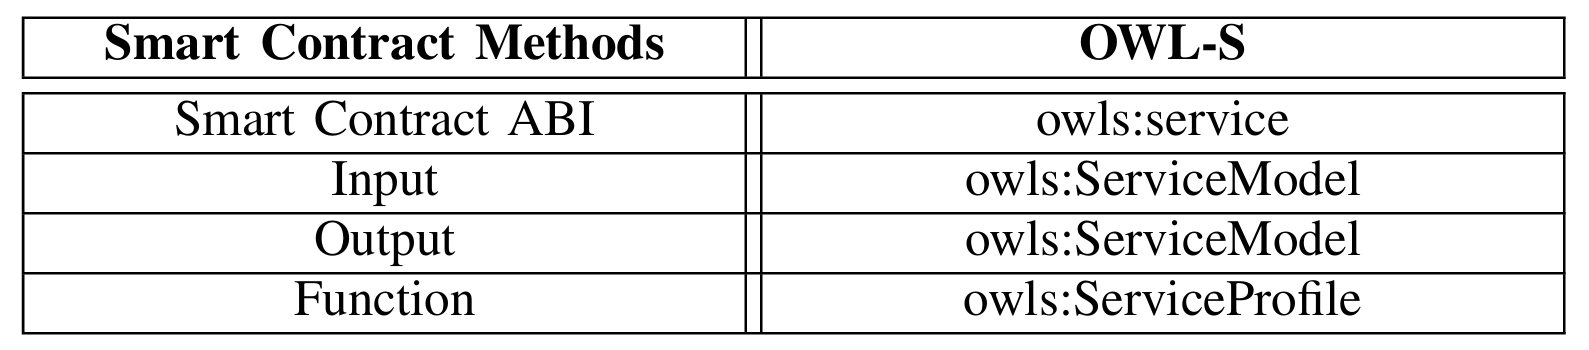
\includegraphics[width=0.7\textwidth]{resources/chapter-2/ssc-ontology-extension.png}
	\caption{Ekstensi OWL-S \parencite{baqa2019semantic}}
	\label{image:ekstensi-owl-s}
\end{figure}

Dalam pengembangan solusi yang diusulkan dalam penelitian ini, dilakukan ekstensi pada OWL-S Service Ontology, seperti pada gambar \ref{image:ekstensi-owl-s} dengan menginkorporasikan beberapa terminologi yang \textit{domain specific} seperti yang ada di dalam EthOn. Sehingga, Semantic Smart Contract dapat digunakan untuk memperkaya query untuk sebuah terminologi yang \textit{domain specific} antar beberapa \textit{distributed ledgers}, yang meningkatkan \textit{discoverability} dari sebuah aplikasi IoT yang terdesentralisasi.
\subsection{Ontological Modeling of Smart Contracts in Solidity}
\label{subsec:solidity-ontology}

Formalisasi menggunakan ontology berbasis domain baru dilakukan pada Blockchain dan Smart Contract, tetapi belum ada yang dilakukan terhadap bahasa pemrograman Smart Contract itu sendiri. Pada penelitiannya, \cite{cano2021toward} mengusulkan sebuah representasi dari bahasa pemrograman Smart Contract yang terkemuka, yaitu Solidity, dengan mendefinisikan semua entitas yang dibutuhkan untuk mencakup seluruh bahasa dan menyelaraskan ke ontology terstandarisasi lainnya seperti EthOn.

Beberapa spesifikasi yang dituliskan di dalam penelitian ini:

\begin{enumerate}
  \item Implementasi Solidity Library
  \item Implementasi Solidity Contract
  \item Interface dan Abstract Contract Solidity
  \item Spesifikasi Attributes dan representasinya di dalam Ontology 
  \item Spesifikasi Types dan representasinya di dalam Ontology
  \item Spesifikasi Constructor dan representasinya di dalam Ontology
  \item Spesifikasi Function dan representasinya di dalam Ontology
  \item Spesifikasi Modifier dan representasinya di dalam Ontology
  \item Spesifikasi Receive dan representasinya di dalam Ontology
  \item Spesifikasi Fallback dan representasinya di dalam Ontology
  \item Spesifikasi Event dan representasinya di dalam Ontology
\end{enumerate}
\subsection{STAN: Towards Describing Bytecodes of Smart Contract}
\label{subsec:stan}

Penelitian yang dilakukan oleh \cite{stan} mengusulkan sebuah sistem bernama STAN untuk melakukan deskripsi terhadap \textit{bytecodes} dari Smart Contracts. STAN merupakan sebuah sistem yang dirancang untuk mengatasi masalah dalam mengekstraksi informasi dari \textit{bytecodes} yang dihasilkan oleh kompilator Solidity. Untuk setiap \textit{interface}, terdapat empat kategori deskripsi yang dapat dihasilkan, yaitu: \textit{functionality description}, \textit{usage description}, \textit{behaviour description}, dan \textit{payment description}. STAN bekerja dengan memanfaatkan \textit{symbolic execution} dan \textit{Natural Language Processing} (NLP) untuk menghasilkan deskripsi yang lebih mudah dipahami oleh pengguna.

\begin{figure}[ht]
	\centering
	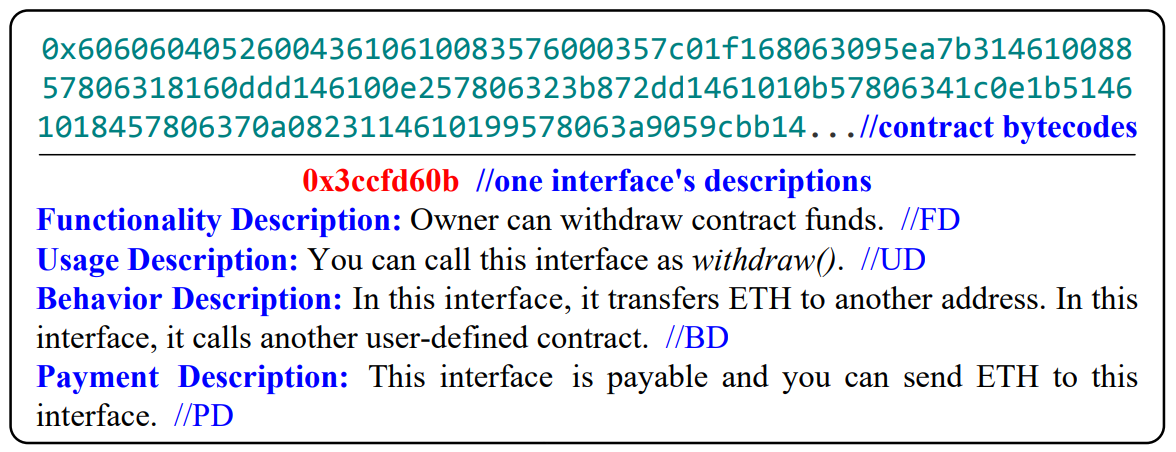
\includegraphics[width=0.7\textwidth]{resources/chapter-2/stan-desc.png}
	\caption{Hasil deskripsi dari STAN untuk Bytecode salah satu \textit{closed-source} Smart Contract \parencite{stan}}
	\label{image:stan-desc}
\end{figure}

\begin{figure}[ht]
	\centering
	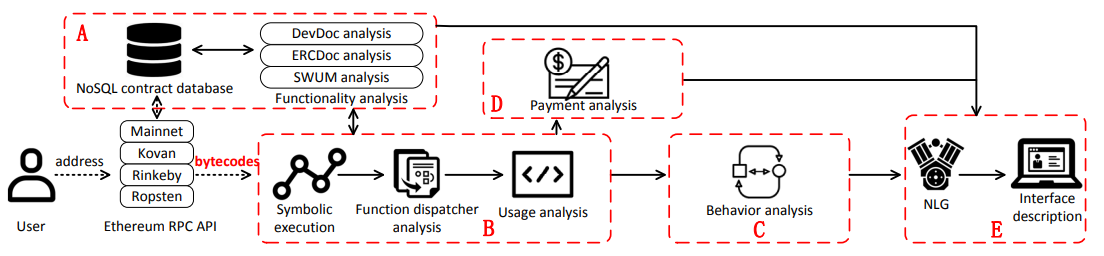
\includegraphics[width=0.7\textwidth]{resources/chapter-2/stan-architecture.png}
	\caption{Arsitektur sistem STAN \parencite{stan}}
	\label{image:stan-architecture}
\end{figure}

Arsitektur dari STAN (Gambar \ref{image:stan-architecture}) terdiri dari beberapa modul utama, yaitu:

\begin{enumerate}
	\item \textbf{Functionality Analysis Module} \\
	      Modul ini melakukan analisis terhadap kontrak melalui teknik \textit{Natural Language Processing} (NLP) untuk menghasilkan frasa yang terkait dengan fungsionalitas dari \textit{interface} kontrak. Fungsionalitas utama dari modul ini adalah untuk mendeskripsikan Bytecode \textit{closed-source contracts}, sementara kontrak \textit{open-source contracts} dan metadata dianalisis untuk membantu analisis Bytecode dengan menemukan \textit{byte signatures} yang identik.

	\item \textbf{Usage Analysis Module} \\
	      Modul ini mengekstrak \textit{byte signatures} fungsi dari \textit{dispatcher} fungsi dan mengembalikan \textit{signature} teks yang sesuai. Dari \textit{signature} teks (misalnya \texttt{transfer(address, uint256)}), pengguna dapat mengetahui nama fungsi dan konfigurasi parameter yang digunakan untuk memanggil \textit{interface}. Modul ini memungkinkan pemahaman yang lebih baik mengenai bagaimana fungsi digunakan dalam kontrak.

	\item \textbf{Behavior Analysis Module} \\
	      Modul ini menganalisis fungsi eksternal/publik untuk menghasilkan informasi perantara terkait perilaku panggilan pesan menggunakan \textit{symbolic execution}. Dengan menganalisis opcode dan operand, modul ini dapat mengenali empat jenis perilaku sensitif dalam panggilan pesan, seperti transfer ETH, penerapan kontrak, dan panggilan kontrak.

	\item \textbf{Payment Analysis Module} \\
	      Modul ini menganalisis fungsi eksternal/publik untuk menghasilkan informasi perantara terkait fitur pembayaran melalui \textit{symbolic execution}. Dengan membangun \textit{Control Flow Graph} (CFG), modul ini dapat mengenali dua pola pembayaran yang menunjukkan apakah \textit{interface} tersebut dapat melakukan pembayaran atau tidak.

	\item \textbf{NLG Module} \\
	      Modul ini menghasilkan deskripsi \textit{interface} yang dapat dibaca dengan memanfaatkan hasil dari empat modul sebelumnya. Proses \textit{Natural Language Generation} (NLG) mengikuti alur standar sistem NLG, yaitu \textit{document planner}, \textit{microplanner}, dan \textit{surface realizer}, untuk menghasilkan deskripsi \textit{interface} yang mudah dipahami oleh pengguna.
\end{enumerate}

STAN dikembangkan pada tahun 2020, dan mencapai hasil yang sangat baik dalam melakukan deskripsi Smart Contract yang bersifat \textit{closed-source}, yang meliputi sekitar 99\% dari seluruh Smart Contracts. Dengan adanya STAN, pengguna dapat memahami fungsionalitas, penggunaan, perilaku, dan pembayaran yang terkait dengan Smart Contract tanpa harus melihat kode sumber dari kontrak tersebut. Hasil deskripsi dari STAN dapat dilihat pada Gambar \ref{image:stan-desc}. STAN adalah sebuah perangkat lunak yang tidak bersifat \textit{open-source} sehingga tidak dapat digunakan secara luas. Namun, konsep yang diusulkan oleh STAN dapat dijadikan sebagai dasar untuk pengembangan sistem yang serupa.

\subsection{Towards a Uniform Description Language for Smart Contract}
\label{subsec:uniform-description-language}

Penelitian yang dilakukan oleh \cite{udlsc} mengusulkan sebuah \textit{Uniform Description Language} untuk Smart Contract bernama UDL-SC yang adalah sebuah ekstensi dari USDL. USDL digunakan untuk mendeskripsikan parameter bisnis, operasional, dan teknikal dari \textit{services} yang ada di Internet, sehingga terdapat informasi lainnya seperti \textit{Service Level Agreement} dan hal lainnya. UDL-SC dibangun di atas USDL karena USDL menyediakan deskripsi yang kaya dan komprehensif yang mendeskripsikan parameter \textit{functional} dan \textit{non-functional}. Tujuan dari UDL-SC adalah untuk meningkatkan akses dan pemahaman mengenai Smart Contract dengan sebuah usulan bahasa deskripsi standar.

\begin{figure}[ht]
	\centering
	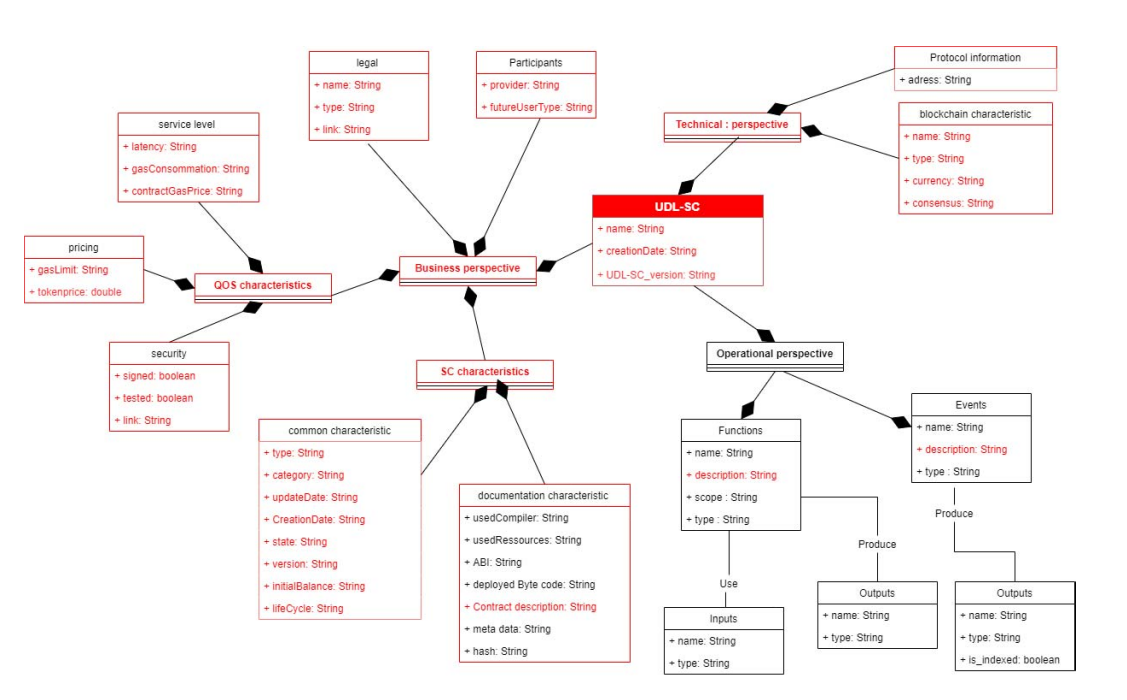
\includegraphics[width=0.7\textwidth]{resources/chapter-2/metamodel-udl-sc.png}
	\caption{Metamodel dari UDL-SC \parencite{udlsc}}
	\label{image:metamodel-udl-sc}
\end{figure}

Metamodel dari UDL-SC dapat dilihat pada Gambar \ref{image:metamodel-udl-sc}. Metamodel dari UDL-SC terdiri dari tiga perspektif utama, yaitu:

\begin{enumerate}
	\item Perspektif Operasional: Berfokus pada atribut fungsional kontrak, seperti fungsi dan event yang dapat dipanggil, beserta parameter yang terlibat.
	\item Perspektif Teknis: Berisi informasi tentang Blockchain tempat kontrak dijalankan, termasuk tipe Blockchain, konsensus, dan protokol yang digunakan.
	\item Perspektif Bisnis: meliputi karakteristik \textit{Quality of Service} (QoS) seperti konsumsi gas, harga gas, serta elemen keamanan dan legal yang terikat pada kontrak, memberikan gambaran yang lebih lengkap dan terperinci mengenai kontrak pintar secara menyeluruh.
\end{enumerate}

\begin{figure}[ht]
	\centering
	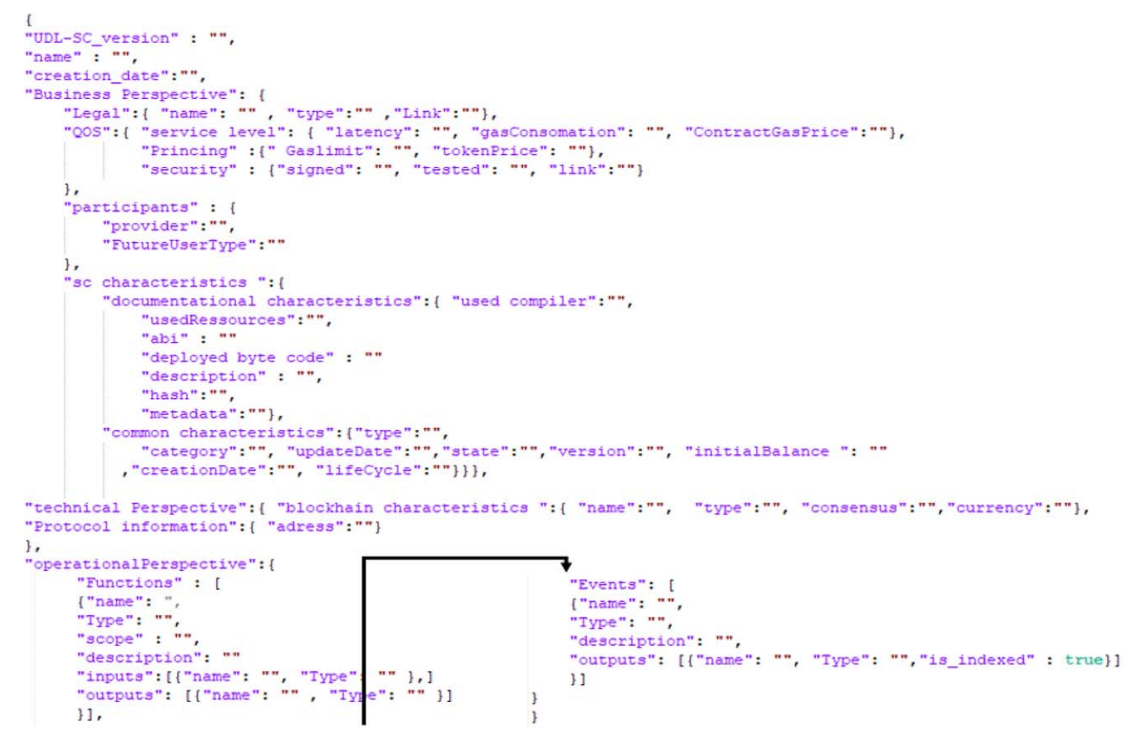
\includegraphics[width=0.7\textwidth]{resources/chapter-2/json-structure-udl-sc.png}
	\caption{Struktur deskripsi umum JSON \parencite{udlsc}}
	\label{image:json-structure-udl-sc}
\end{figure}

Gambar \ref{image:json-structure-udl-sc} menunjukkan deskripsi umum dari struktur UDL-SC dalam format JSON. Dalam penelitian ini, skema JSON dibangkitkan secara otomatis menggunakan kelas Java \texttt{SchemaGenerator}. Proses pembangkitan skema JSON ini dideskripsikan dalam gambar \ref{image:schema-generation-udl-sc}.

\begin{figure}[ht]
	\centering
	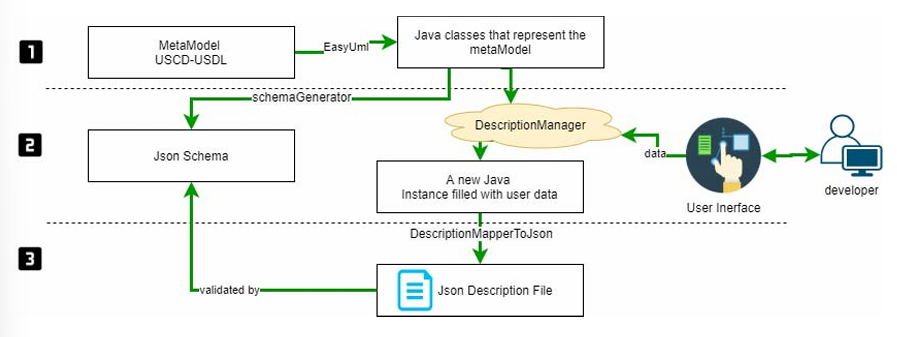
\includegraphics[width=0.7\textwidth]{resources/chapter-2/schema-generation-udl-sc.png}
	\caption{Proses pembangkitan skema JSON \parencite{udlsc}}
	\label{image:schema-generation-udl-sc}
\end{figure}

\subsection{Supporting Reuse of Smart Contracts through Service Orientation and Assisted Development}
\label{subsec:supporting-reuse-smart-contracts}

Penelitian yang dilakukan oleh \cite{guida2019supporting} membahas tantangan utama yang dihadapi pengembang saat menggunakan kembali Smart Contracts, yaitu kesulitan dalam mencari informasi yang dapat ditindaklanjuti tentang kontrak yang ada dan menulis logika integrasi untuk memanggil kontrak-kontrak yang dipilih serta mengimplementasikan fungsi yang hilang. Penelitian ini mengusulkan format deskripsi Smart Contracts yang memungkinkan pengembang untuk mencari kontrak yang tersedia secara publik, memahami fitur yang diekspos oleh kontrak tersebut, dan bagaimana cara memanggilnya dengan pendekatan berbasis layanan. Untuk mengatasi masalah integrasi, penelitian ini mengimplementasikan lingkungan pengembangan berbasis model yang terdiri dari editor pemrograman visual yang menyediakan sekumpulan konstruksi pemodelan untuk mengenkripsi pola kode yang berfokus pada penggunaan kembali Smart Contracts. Pendekatan ini diimplementasikan dan diuji pada platform Blockchain Ethereum dengan bahasa pemrograman Solidity.

\begin{figure}[ht]
	\centering
	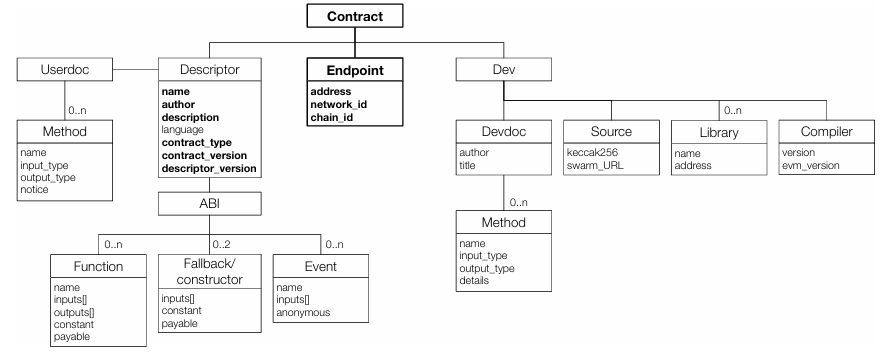
\includegraphics[width=1\textwidth]{resources/chapter-2/sc-model.png}
	\caption{Model deskripsi kontrak \parencite{guida2019supporting}}
	\label{image:sc-model}
\end{figure}

\begin{figure}[ht]
	\centering
	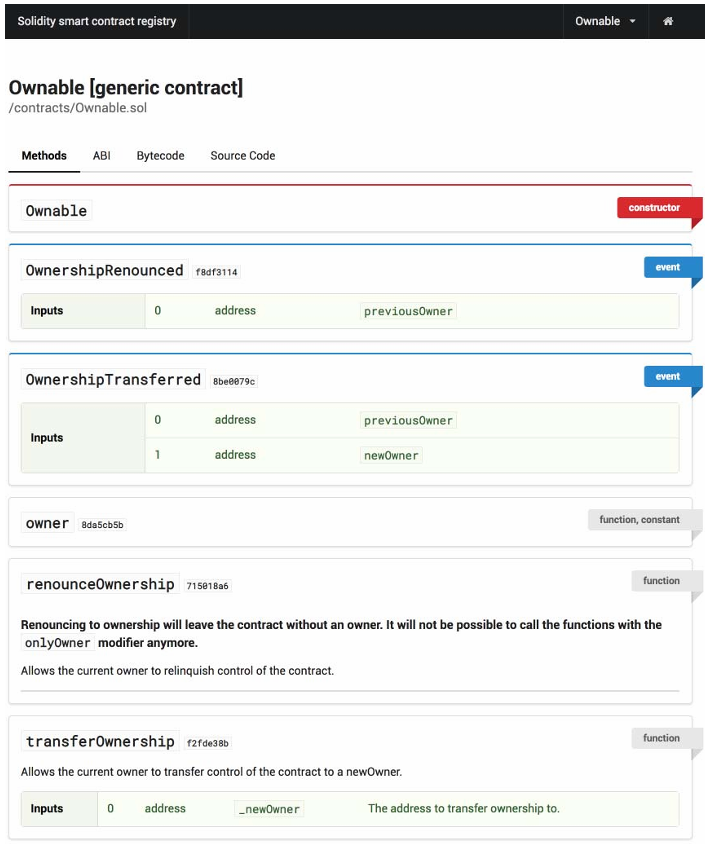
\includegraphics[width=0.7\textwidth]{resources/chapter-2/sc-registry.png}
	\caption{Tampilan Smart Contracts Registry \parencite{guida2019supporting}}
	\label{image:sc-registry}
\end{figure}

\begin{figure}[ht]
	\centering
	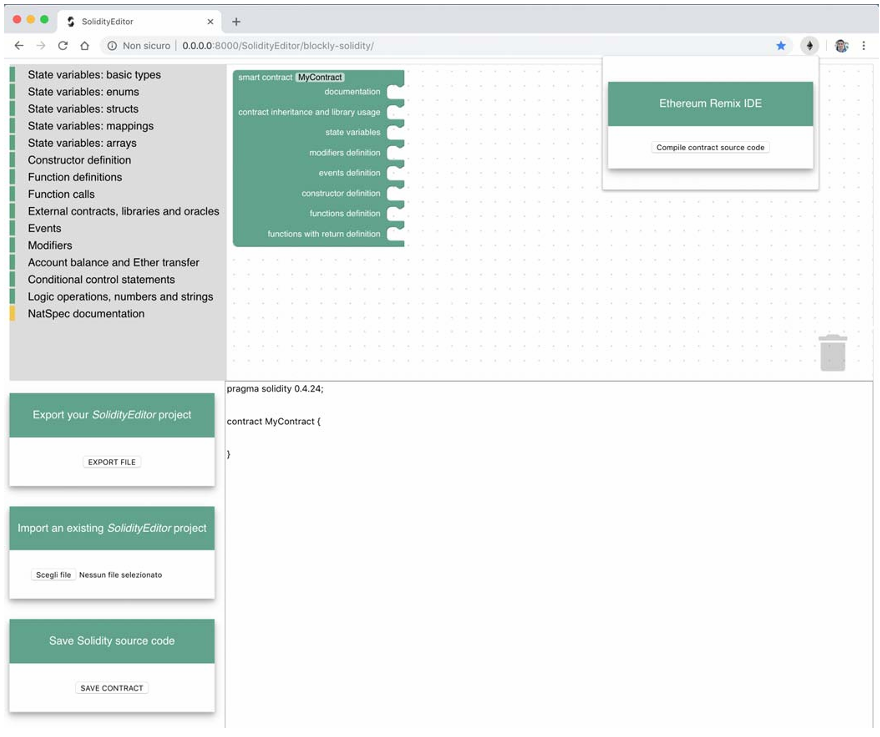
\includegraphics[width=0.7\textwidth]{resources/chapter-2/sc-editor.png}
	\caption{Tampilan Smart Contracts Visual Editor \parencite{guida2019supporting}}
	\label{image:sc-editor}
\end{figure}

\begin{figure}[ht]
	\centering
	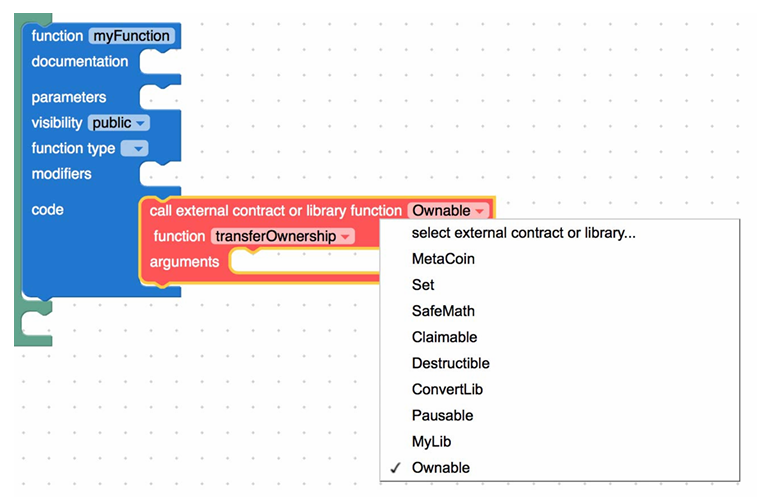
\includegraphics[width=0.7\textwidth]{resources/chapter-2/sc-editor-edit.png}
	\caption{Tampilan Smart Contract Selector \parencite{guida2019supporting}}
	\label{image:sc-editor-edit}
\end{figure}

\break

Penelitian ini menyoroti pentingnya deskripsi Smart Contracts yang memungkinkan pengembang untuk mencari dan menggunakan kontrak yang ada tanpa harus membaca kode sumbernya secara langsung. Model deskripsi kontrak yang diusulkan pada gambar \ref{image:sc-model} mencakup metadata yang sudah ada, seperti ABI dan dokumentasi, serta informasi teknis tambahan untuk memfasilitasi pencarian dan integrasi Smart Contracts. Selain itu, penelitian ini mengembangkan \textit{registry} Smart Contracts seperti yang ditunjukkan pada gambar \ref{image:sc-registry} dan \textit{editor} visual berbasis blok seperti yang ditunjukkan pada gambar \ref{image:sc-editor} dan gambar \ref{image:sc-editor-edit} untuk memudahkan pengembangan Smart Contracts yang lebih besar dan kompleks dengan cara yang lebih efisien dan dapat mengurangi kesalahan pemrograman.

\break

Implementasi ini menunjukkan bahwa penggunaan pendekatan berbasis visual, seperti \textit{editor} SolidityEditor, dapat mengurangi risiko kesalahan sintaksis, mempercepat pengembangan, dan memudahkan penggunaan kembali kode dengan mengintegrasikan pustaka kontrak eksternal seperti yang digunakan dalam studi kasus SmartTrainInsurance.

\newpage
% llm with source code
\subsection{Smart Contracts and Solidity Code Summarization}
\label{subsec:smart-contract-solidity-summary}

Penelitian yang dilakukan oleh \cite{zhang2021smart} membahas tantangan dalam pemrograman dan pemahaman kode Smart Contracts, khususnya pada platform Ethereum, yang sebagian besar menggunakan bahasa pemrograman Solidity. Masalah utama yang dihadapi adalah kurangnya dokumentasi pada kode Smart Contracts, yang menghambat pemahaman bagi pengembang, terutama yang masih pemula dalam pengembangan Smart Contracts. Dalam penelitian ini, penulis mengusulkan sistem yang dinamakan SoliditySummarizer untuk menghasilkan komentar otomatis untuk kode Solidity, guna membantu pengembang, baik yang berpengalaman maupun pemula, dalam memahami dan mendokumentasikan kode Smart Contracts secara lebih mudah.

Pada bagian pertama dari tesis ini, penulis menjelaskan tentang Blockchain dan Ethereum, dengan fokus pada kemampuan Ethereum untuk menjalankan Smart Contracts yang otomatis, terdesentralisasi, dan dapat dieksekusi tanpa pengawasan pihak ketiga. Penelitian ini juga menggali masalah terkait \textit{readability} dan dokumentasi yang sering kali tidak ada pada kode Smart Contracts, serta bagaimana masalah ini dapat diselesaikan dengan menggunakan SoliditySummarizer.

SoliditySummarizer didesain untuk menghasilkan ringkasan dari kode sumber Smart Contracts, dengan menggunakan pendekatan \textit{transformer models} dalam teknik \textit{Natural Language Generation} (NLG). Salah satu elemen penting dalam penelitian ini adalah pembuatan dataset yang digunakan untuk melatih model, yang dikumpulkan dan dibersihkan dari kontrak-kontrak yang terdapat di Etherscan dan GitHub. Selanjutnya, sistem ini menggunakan model berbasis \textit{Transformer} untuk menghasilkan deskripsi yang dapat membantu pengembang memahami fungsi dan struktur kode Solidity.

Dalam bab kedua, penulis mengulas \textit{state of the art} dalam teknologi \textit{code summarization} untuk Smart Contracts, serta menyoroti tantangan yang dihadapi saat menerapkan \textit{machine learning} dalam \textit{summarization} kode, khususnya dalam bahasa Solidity. SMTranslator adalah salah satu alat yang dikaji sebagai perbandingan, namun alat ini memiliki keterbatasan dalam hal akurasi dan fleksibilitas dalam menghasilkan deskripsi yang sesuai dengan kompleksitas Smart Contracts.

SoliditySummarizer menggunakan teknik yang lebih canggih, termasuk \textit{multi-head self-attention networks} dan penggunaan \textit{pre-trained models} untuk mengatasi kekurangan data pelatihan yang terbatas. Hasil evaluasi menunjukkan bahwa SoliditySummarizer lebih unggul dibandingkan alat sebelumnya, terutama dalam hal \textit{accuracy} dan \textit{conciseness}, meskipun masih ada tantangan dalam \textit{readability} dari komentar yang dihasilkan.

Penelitian ini menekankan bahwa meskipun SoliditySummarizer memberikan hasil yang lebih baik dibandingkan dengan metode berbasis template sebelumnya, tantangan terbesar terletak pada \textit{readability} komentar yang dihasilkan, yang cenderung terlalu teknis dan sulit dipahami bagi \textit{non-programmer}. SoliditySummarizer tetap memberikan kontribusi besar dalam meningkatkan pemahaman dan penggunaan Smart Contracts di platform Ethereum, serta membuka kemungkinan penggunaan \textit{machine learning} untuk meningkatkan dokumentasi otomatis di masa depan.

% pencarian dan rekomendasi
% langchain
\subsection{Semantic Code Search for Smart Contracts}
\label{subsec:semantic-code-search}

Penelitian yang dilakukan oleh \cite{shi2021semantic} mengusulkan model pencarian kode semantik untuk kontrak pintar yang disebut MM-SCS (Multi-Modal Smart Contract Code Search). Model ini dirancang untuk mengatasi masalah yang sering ditemui pada teknik pencarian kode tradisional, yaitu adanya jarak semantik antara kode dan query yang menghambat efektivitas pencarian. Penelitian ini berfokus pada pengembangan model pencarian kode yang tidak hanya menggunakan representasi teks dari kode, tetapi juga memasukkan informasi alur kontrol dan data, yang sangat penting dalam konteks kontrak pintar yang kompleks.

\begin{figure}[ht]
  \centering
  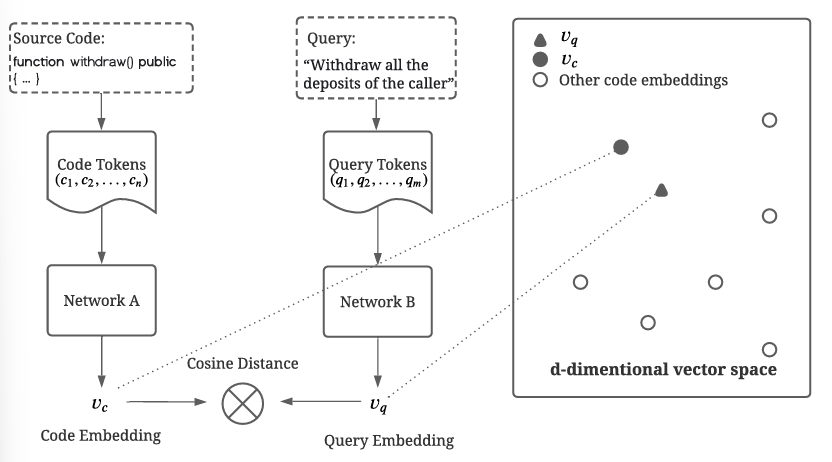
\includegraphics[width=0.7\textwidth]{resources/chapter-2/architecture-code-search.png}
  \caption{Arsitektur umum dari Neural Code Search \parencite{shi2021semantic}}
  \label{image:architecture-code-search}
\end{figure}

Dalam penelitian ini, MM-SCS mengintegrasikan Contract Elements Dependency Graph (CEDG) sebagai modalitas tambahan untuk menangkap informasi tentang alur data dan kontrol dalam kode. CEDG menggambarkan elemen-elemen utama dalam kode kontrak pintar, seperti variabel, fungsi, dan hubungan antar elemen tersebut, serta bagaimana elemen-elemen ini saling berinteraksi dalam kontrak pintar. Model ini juga mengadopsi teknik multi-head attention network untuk menghasilkan embedding dari fitur kode, yang memungkinkan model lebih fokus pada informasi konteks yang penting dalam kode.

Untuk memastikan efektivitas model meskipun data pelatihan terbatas, penulis menggunakan model ALBERT yang sudah dilatih sebelumnya dan disesuaikan untuk meningkatkan pemahaman konteks kode dalam pencarian semantik. Hasil eksperimen yang dilakukan menggunakan dataset yang berisi 470.000 pasangan kode dan deskripsi dari Github dan Etherscan menunjukkan bahwa MM-SCS mengungguli empat model state-of-the-art lainnya dalam hal Mean Reciprocal Rank (MRR) dan waktu pencarian, dengan peningkatan yang signifikan dalam akurasi pencarian kode pintar.

\begin{figure}[ht]
  \centering
  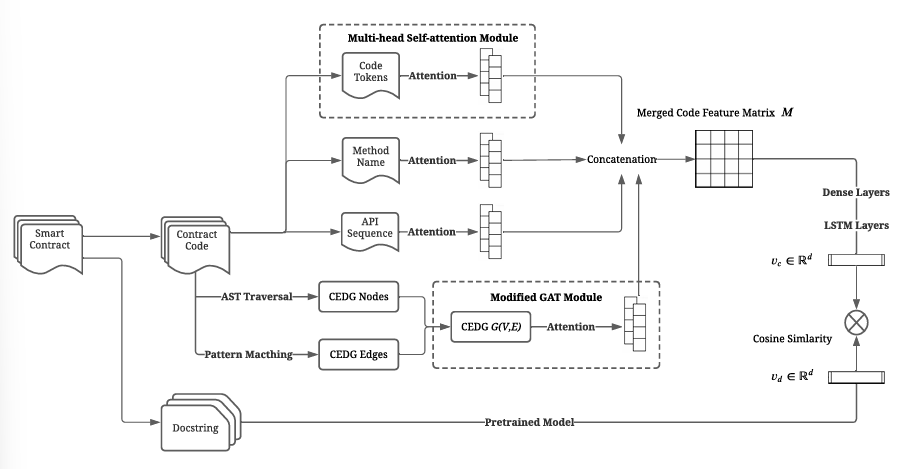
\includegraphics[width=0.7\textwidth]{resources/chapter-2/framework-mm-scs.png}
  \caption{Framework keseluruhan dari MM-SCS \parencite{shi2021semantic}}
  \label{image:framework-mm-scs}
\end{figure}

Penelitian ini memberikan kontribusi penting dalam meningkatkan pencarian kode semantik untuk Smart Contracts dengan memperkenalkan CEDG sebagai representasi grafis yang menggambarkan hubungan antar elemen kode dan menambahkan modalitas graf dalam pencarian semantik. Riset ini membuktikan bahwa CEDG lebih efektif untuk dijadikan modalitas tambahan dibandingkan dari AST. Selain itu, eksperimen ini menunjukkan bahwa pendekatan MM-SCS memiliki keunggulan dibandingkan dengan model-model lainnya dalam hal akurasi dan efisiensi pencarian, walaupun dengan \textit{training time cost} yang lebih tinggi.

Hasil dari penelitian ini diharapkan dapat meningkatkan efisiensi pengembangan Smart Contracts dengan mempermudah pencarian dan penggunaan kembali potongan kode yang relevan dari repositori besar kode Smart Contracts.
